\section{Metodi non lineari}\label{sec:non-linear}

Nella sezione \ref{sec:linear-model} sono stati introdotti ed adottati dei
metodi di regressione lineare che fornivano dei risultati discreti in prima
analisi, ma che possono essere sostituiti con modelli non lineari che spiegano
ancora meglio i dati.

A tal fine, sono stati provati vari modelli, descritti nelle sottosezioni
seguenti.

%%%%%%%%%%%%%%%%%%%%%%%%%%%%%%%%%%%%%%%%%%%%%%%%%%%%%%%%%%%%%%%%%%%%%%%%%%%%%%%

\subsection{Regressione locale}\label{sec:local-regression}
Come primo modello non lineare si sceglie di utilizzare la regressione locale,
servendosi del package \texttt{sm} presente in R.

In questo caso ci si limita a eseguire la regressione locale solamente per le
due variabili \texttt{datetime} e \texttt{temp}, le quali ci si aspettava che
fossero più importanti per la richiesta del servizio di \emph{Bike sharing};
tale ipotesi è stata verificata grazie al modello lineare, in cui queste
variabili erano risultate più significative sia nella scala logaritmica che in
quella originale.

Oltre a questo, la regressione locale viene svolta solamente per la scala
logaritmica, poichè si ritiene che riesca a modellare meglio il sistema in
esame.

\paragraph{Scelta di \emph{h}} \mbox{}\\
Per questo modello era importante scegliere il parametro \emph{h}, che regola
l'ampiezza della finestra di lisciamento.

Per la scelta del parametro, gli script \texttt{mySM\_temp.R} (sez.
\ref{sec:mySM-temp}) e lo script \texttt{mySM\_datetime.R} (non riportato
perchè pressochè uguale a quello per la variabile \texttt{temp}) sono stati
fatti girare più volte, ottenendo ogni volta una misura ottimale di h e
restringendo l'intervallo attorno al valore salvato in \texttt{optimal\_h}.

Di seguito viene riportato l'andamento dell'errore in funzione di h:

\begin{figure}[H]
  \centering
  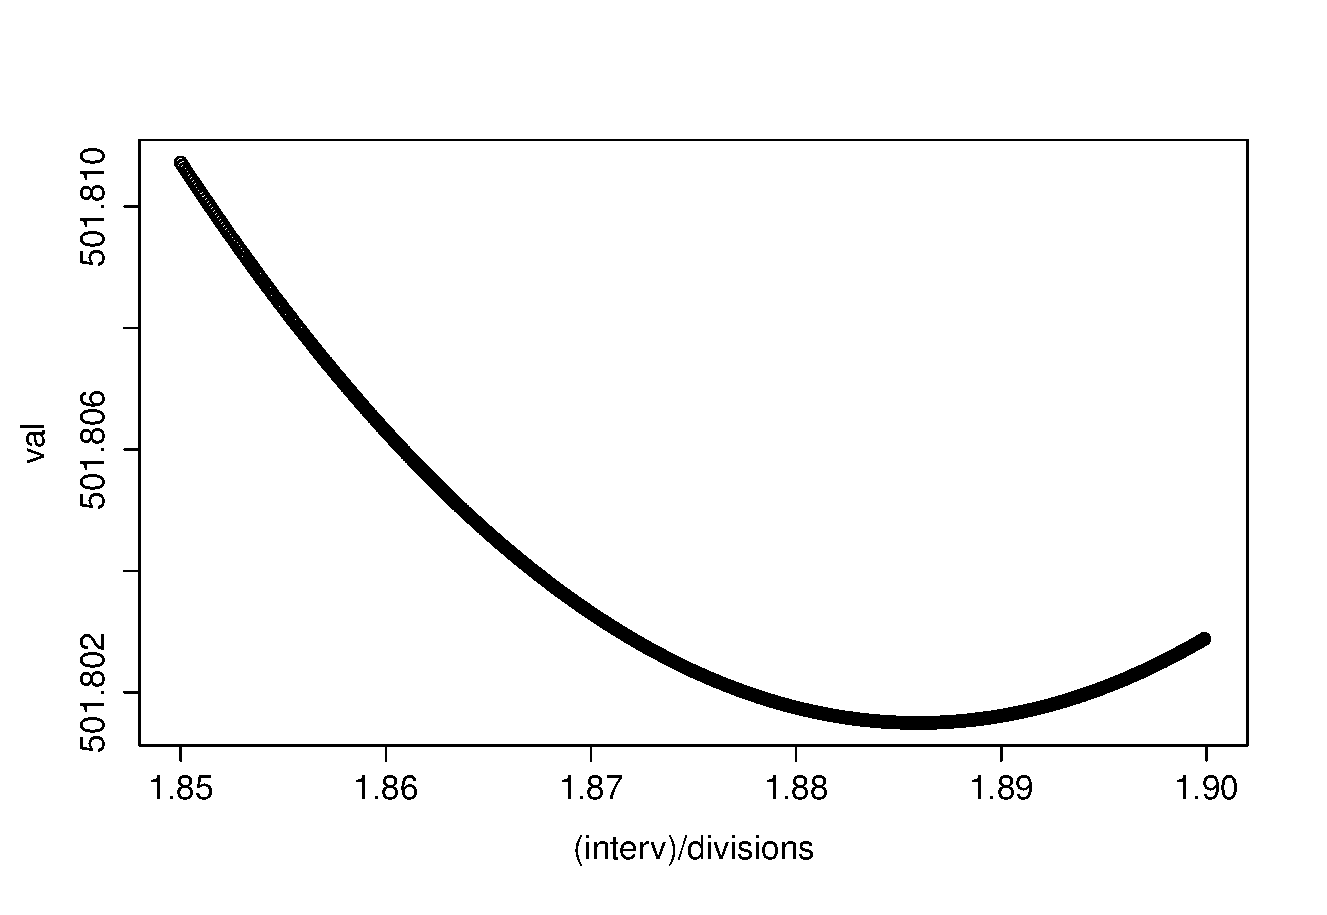
\includegraphics[width=.7\columnwidth]{images/non-linear/sm-optimal-h.eps}
  \caption{Curva dell'errore in funzione del parametro h}
  \label{fig:sm-optimal-h}
\end{figure}

Una volta iterato il procedimento fino ad avere una precisione per l'h
``ottimo'' migliore di $ \frac{1}{1000} $, si procede a disegnare la curva
grazie allo script \texttt{drawOptimalSM\_temp.R} (sez. \ref{sec:drawSM-temp}):

\begin{figure}[H]
  \centering
  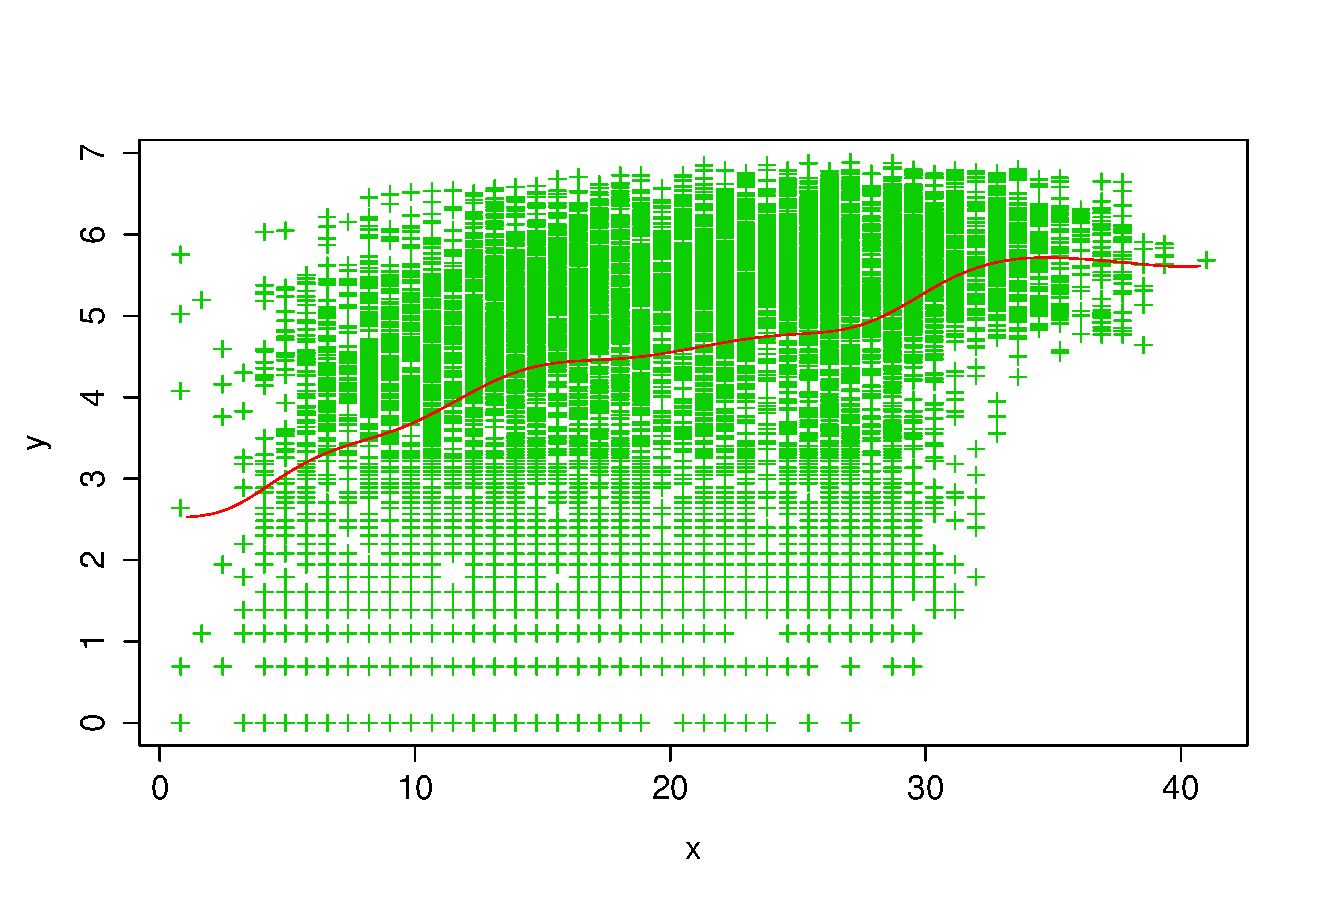
\includegraphics[width=.7\columnwidth]{images/non-linear/sm-draw.eps}
  \caption{Curva di regressione locale disegnata con il miglior h}
  \label{fig:sm-draw}
\end{figure}

%%%%%%%%%%%%%%%%%%%%%%%%%%%%%%%%%%%%%%%%%%%%%%%%%%%%%%%%%%%%%%%%%%%%%%%%%%%%%%%

\subsection{Loess}\label{sec:loess}
Un metodo molto simile al precedente, sempre di regressione locale, è il
\emph{loess}.

Questa tecnica permette di attenuare gli effetti degli \emph{outliers}, poichè
considera un intorno di k \emph{punti} e non un intorno di \emph{ampiezza} h.
Grazie a questa sua particolarità, il \emph{loess} è ritenuto un estimatore
\textbf{robusto}.

Tuttavia, anche questa tecnica viene eseguita con poche variabili alla volta;
sebbene il numero massimo di \emph{covariates} che il comando \texttt{loess}
di R accetta sia 4, si ritiene che eseguire la regressione locale con una
sola variabile esplicativa ne favorisca interpretazione.

Gli script utilizzati sono \texttt{loess\_temp.R} (sez. \ref{sec:loess-temp})
ed altri script non riportati perchè sostanzialmente identici a questo. In
tali procedure viene generato un insieme di addestramento e uno di verifica,
per poi cercare l'\texttt{optimal\_span} (la percentuale per la quale la somma
dei quadrati dei residui è minima).

\begin{figure}[H]
  \centering
  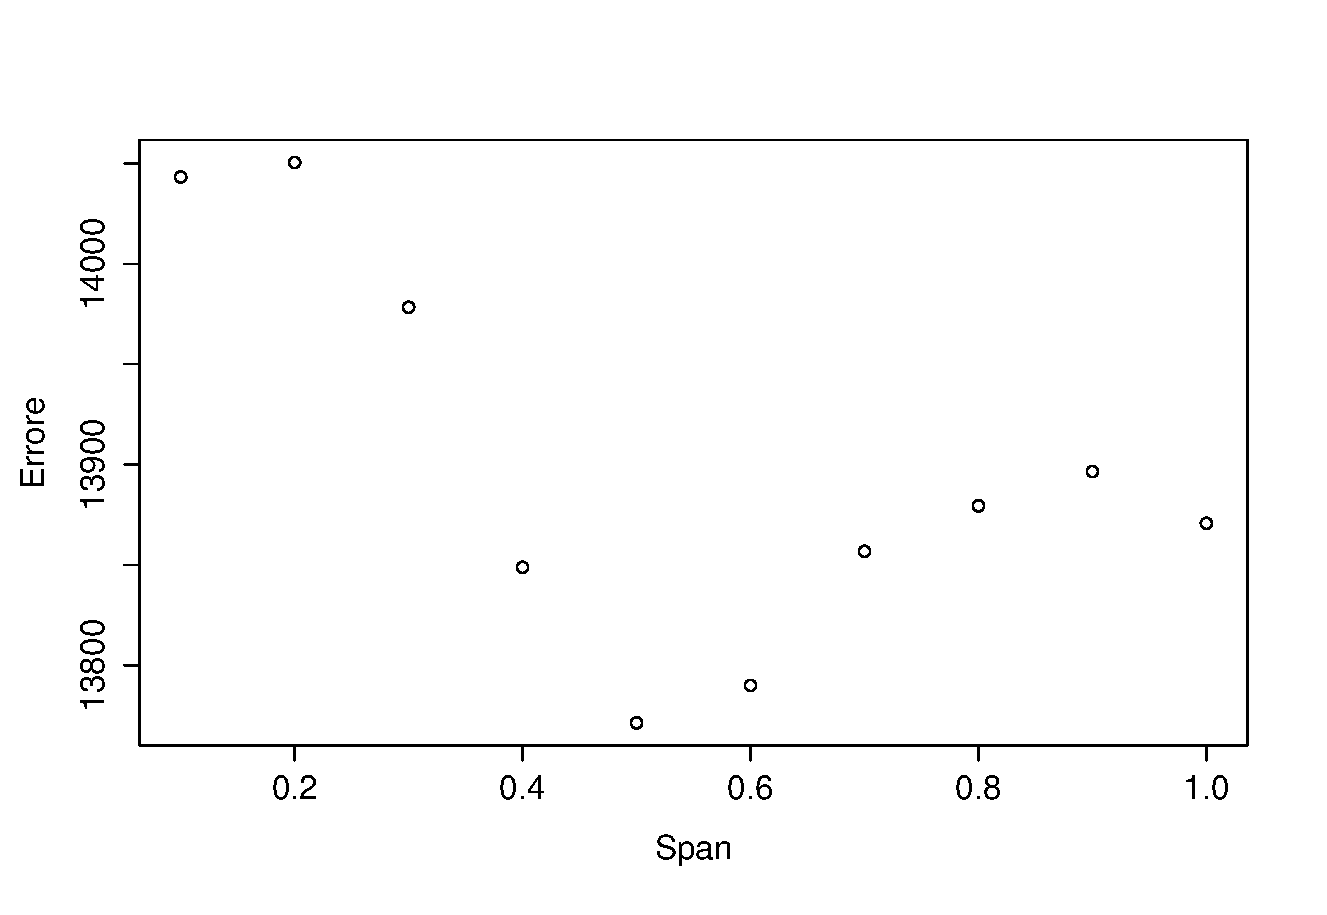
\includegraphics[width=.7\columnwidth]{images/non-linear/loess-error-span.eps}
  \caption{Curva dell'errore in funzione del parametro span}
  \label{fig:loess-optimal-span}
\end{figure}

\begin{figure}[H]
  \centering
  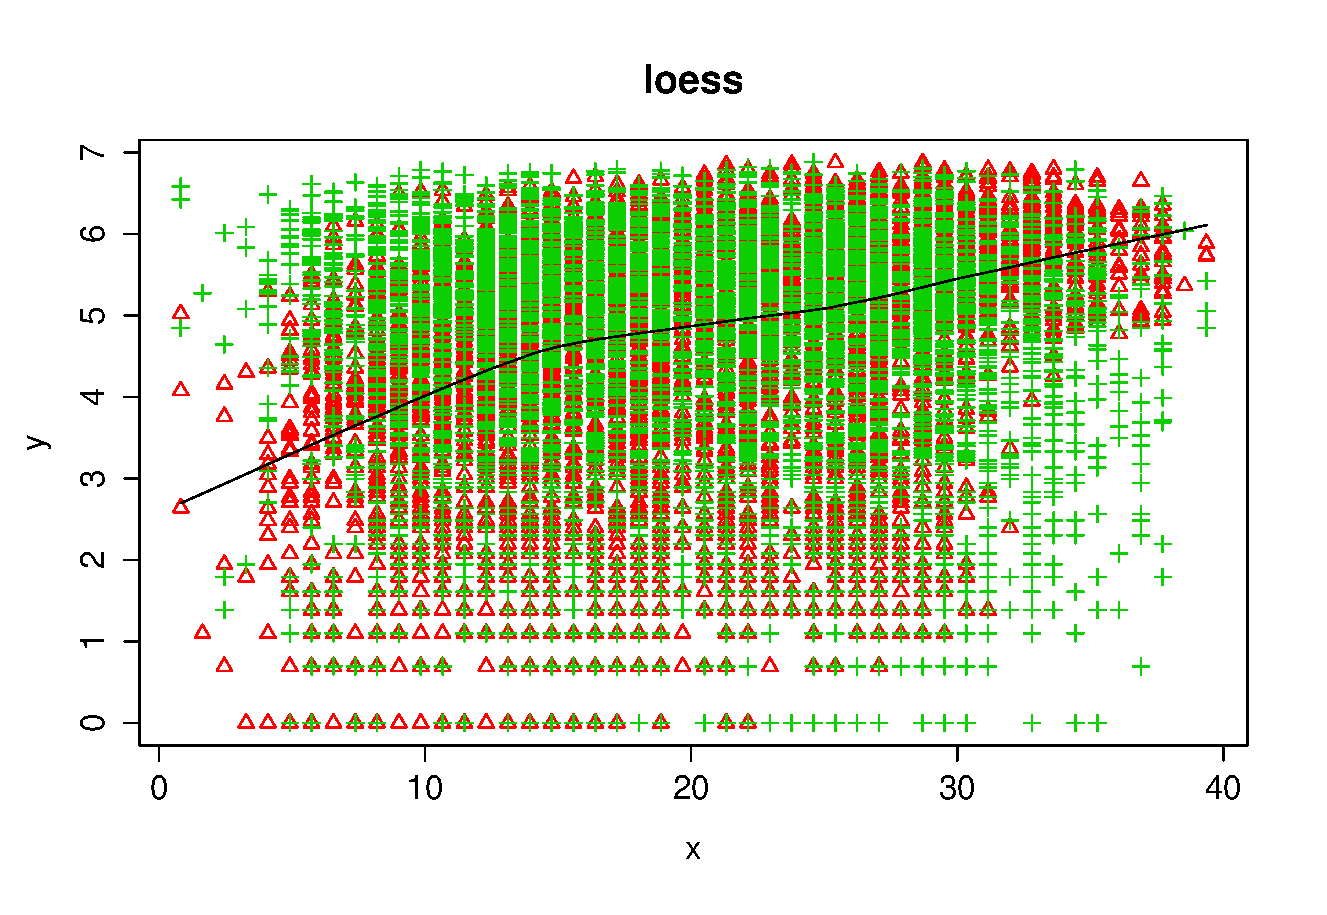
\includegraphics[width=.7\columnwidth]{images/non-linear/loess-draw.eps}
  \caption{Curva loess disegnata con il miglior span}
  \label{fig:loess-draw}
\end{figure}

%%%%%%%%%%%%%%%%%%%%%%%%%%%%%%%%%%%%%%%%%%%%%%%%%%%%%%%%%%%%%%%%%%%%%%%%%%%%%%%

\subsection{Spline di regressione}\label{sec:regression-splines}
Finora sono stati usati solamente modelli che, lineari o meno, erano costituiti
da una o più rette di regressione.

Con le spline si passa a curve che hanno tratti definiti da polinomi di grado
maggiore al primo: più precisamente, nel nostro caso verranno utilizzate
spline cubiche (con tratti definiti da polinomi di terzo grado).

Gli script che realizzano queste curve sono \texttt{regression-splines-temp.R}
(sez. \ref{sec:regression-splines-temp}) ed altri script non riportati perchè
sostanzialmente identici a questo.

Tali procedure utilizzano il comando \texttt{bs} di R, che genera spline con la
possibilità di impostare grado e numero di nodi.

\begin{figure}[H]
  \centering
  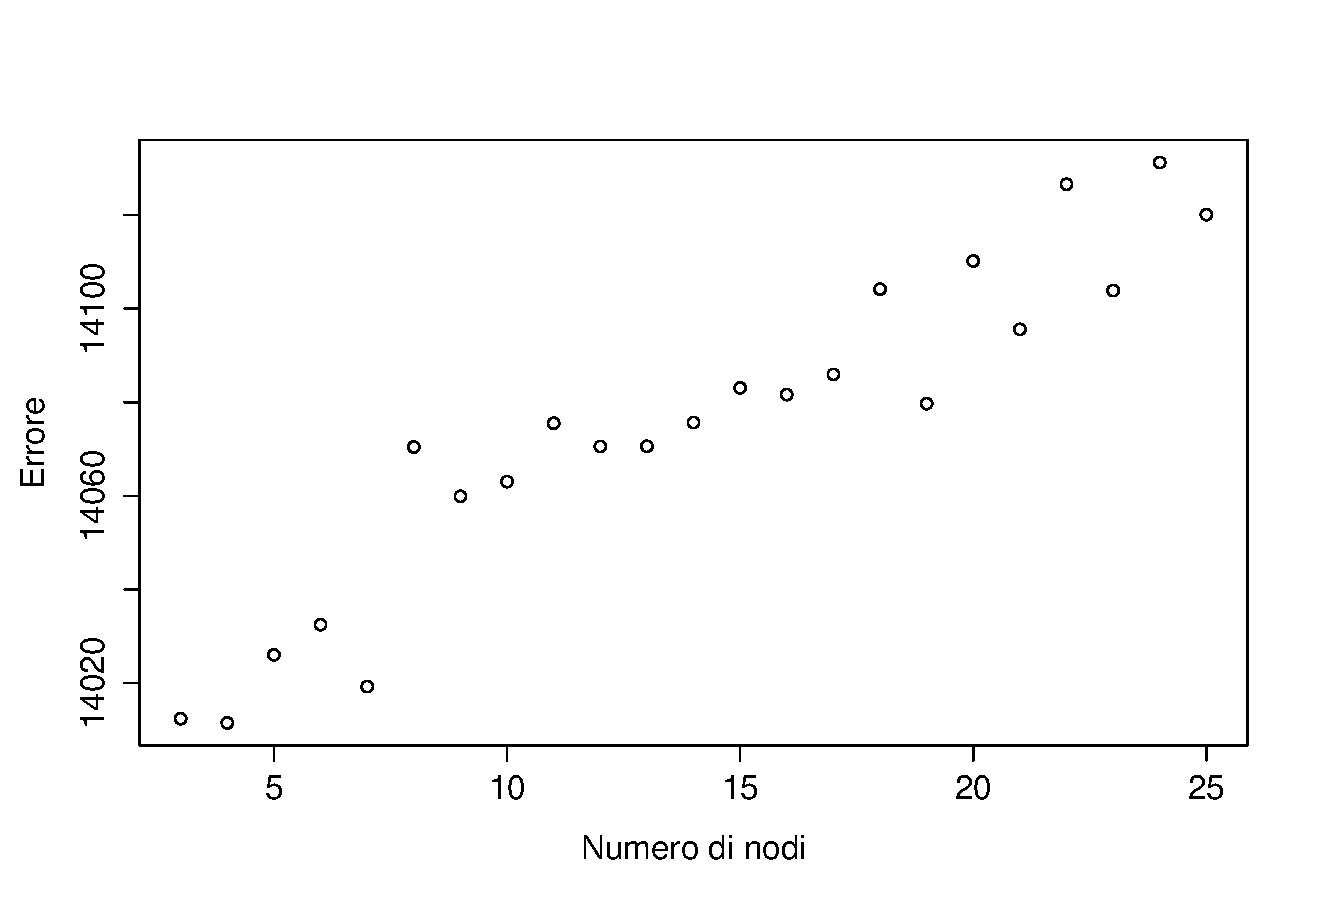
\includegraphics[width=.7\columnwidth]{images/non-linear/regression-splines-error-knots.eps}
  \caption{Curva dell'errore in funzione del numero di nodi}
  \label{fig:regression-optimal-knots}
\end{figure}

\begin{figure}[H]
  \centering
  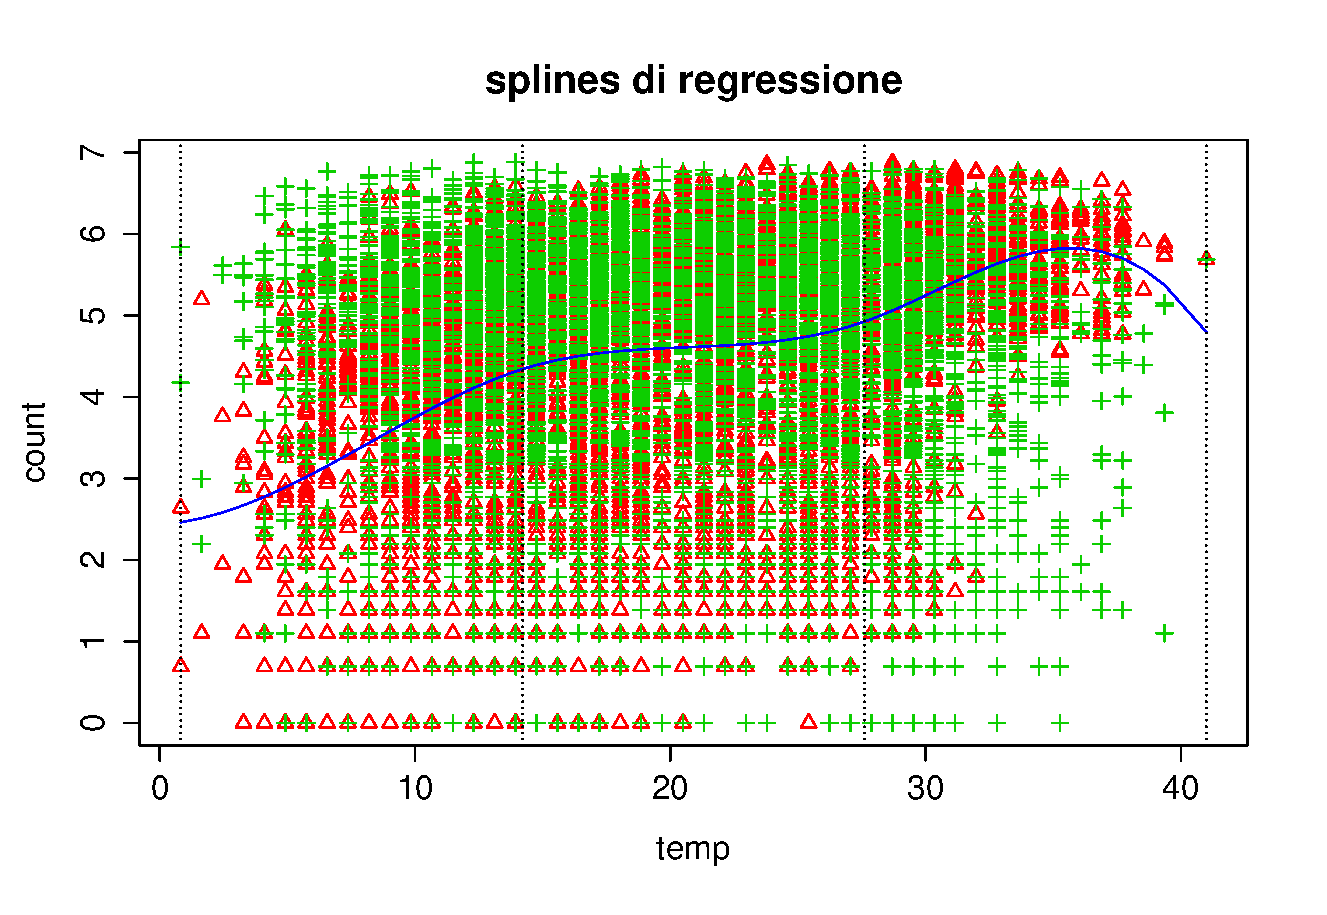
\includegraphics[width=.7\columnwidth]{images/non-linear/regression-draw.eps}
  \caption{Spline di regressione disegnata con il miglior numero di nodi}
  \label{fig:regression-draw}
\end{figure}

%%%%%%%%%%%%%%%%%%%%%%%%%%%%%%%%%%%%%%%%%%%%%%%%%%%%%%%%%%%%%%%%%%%%%%%%%%%%%%%

\subsection{Spline di lisciamento}\label{sec:smoothing-splines}
A differenza delle spline di regressione, che agivano sull'intera funzione,
possiamo anche introdurre un modello di regressione locale non lineare, ovvero
le \emph{spline di lisciamento}.

In un modo simile a quello visto per le spline di regressione, vengono
ottenute tante spline, una per ognuno degli intervalli scelti.

In questo caso, gli script utilizzati per ottenere il relativo modello sono
\texttt{smoothing-splines-temp.R} (sez. \ref{sec:smoothing-splines-temp}) ed
altri script non riportati perchè sostanzialmente identici a questo.

Tali procedure iterano affinchè non viene trovato il miglior valore di
$ \lambda $, ovvero il parametro di lisciamento utilizzato per tale modello (
$ \lambda = 0 \rightarrow $ funzione frastagliata,
$ \lambda = \infty \rightarrow $ regressione lineare semplice).

\begin{figure}[H]
  \centering
  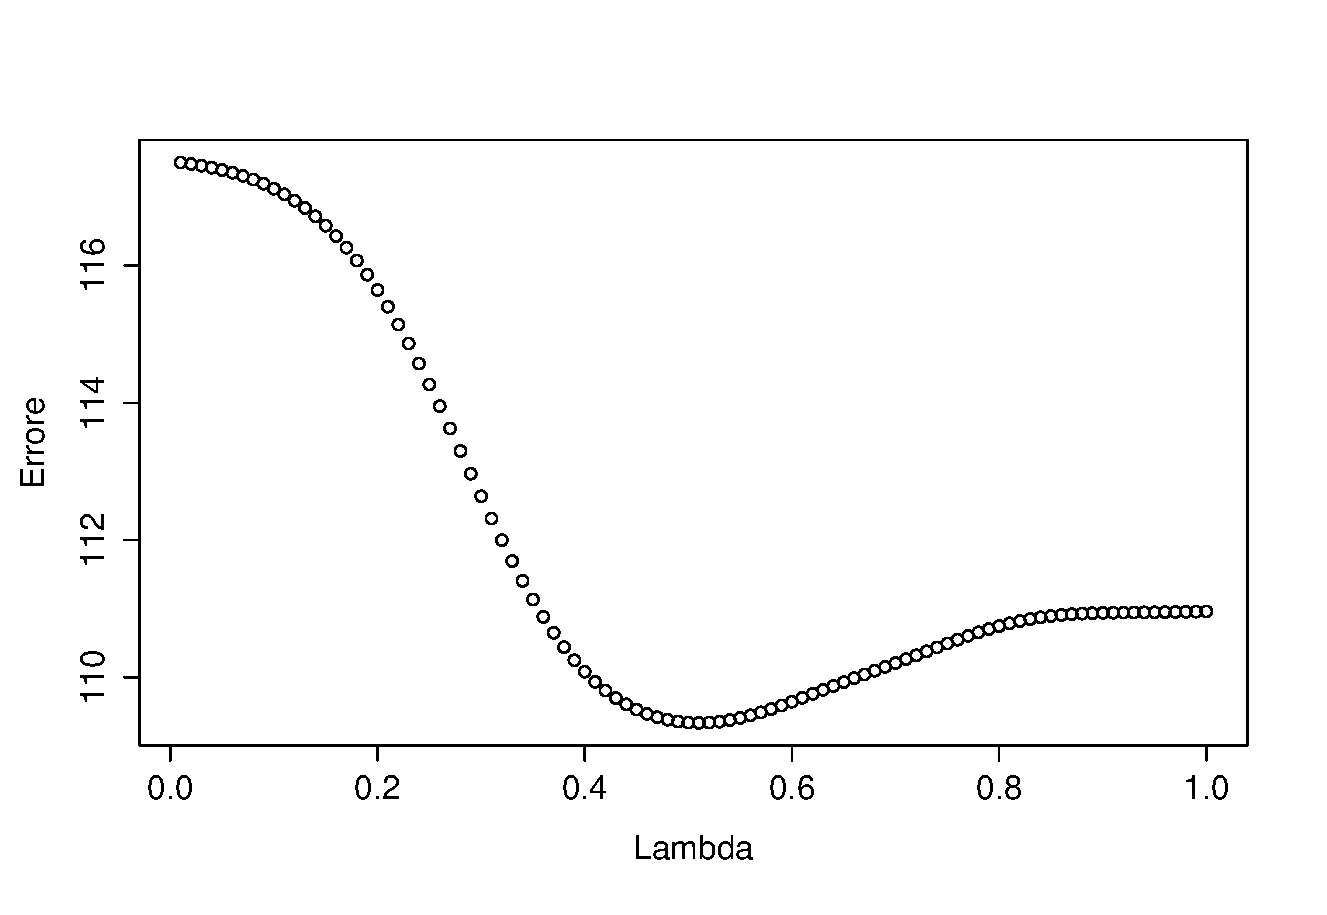
\includegraphics[width=.7\columnwidth]{images/non-linear/smoothing-splines-error-lambda.eps}
  \caption{Curva dell'errore in funzione di $ \lambda $}
  \label{fig:smoothing-optimal-lambda}
\end{figure}

\begin{figure}[H]
  \centering
  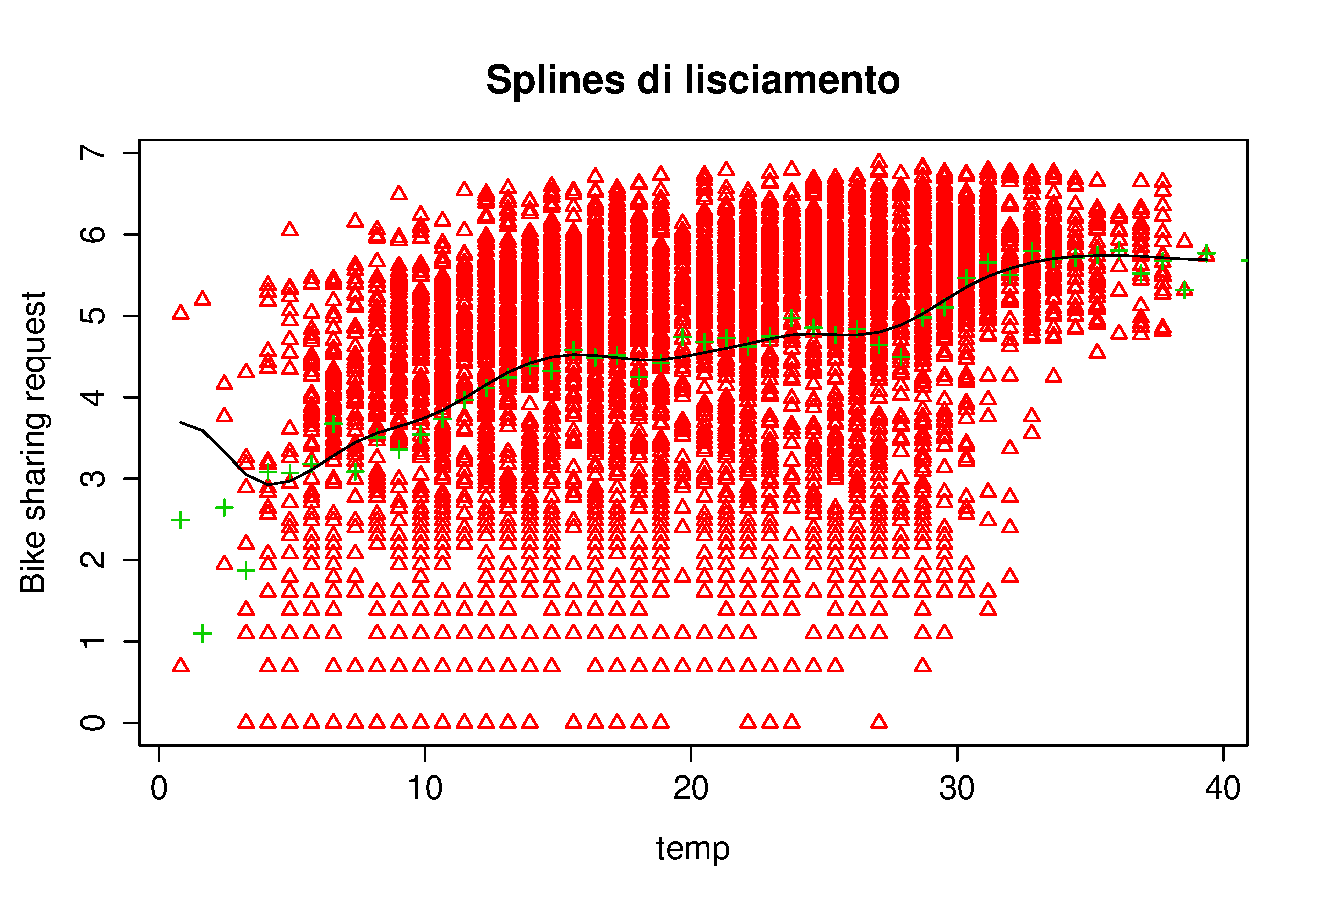
\includegraphics[width=.7\columnwidth]{images/non-linear/smoothing-spl-draw.eps}
  \caption{Spline di lisciamento disegnata con il miglior $ \lambda $}
  \label{fig:smoothing-spline-draw}
\end{figure}

%%%%%%%%%%%%%%%%%%%%%%%%%%%%%%%%%%%%%%%%%%%%%%%%%%%%%%%%%%%%%%%%%%%%%%%%%%%%%%%

\subsection{MARS}\label{doc:smoothing-splines}
Oltre alle tecniche viste nelle sezioni \ref{sec:regression-splines} e
\ref{sec:smoothing-splines} vi è un ulteriore tecnica che utilizza le spline,
ovvero MARS (\emph{Multivariate Adaptive Regression Splines}).

Come dice il nome (esteso), grazie a questa tecnica è possibile utilizzare le
splines di regressione non solo più con un'unica variabile, ma con tutte le
variabili esplicative del dataset.

Lo script utilizzato per MARS è \texttt{mars.R}, presente in sezione
\ref{sec:mars-script}.
